\documentclass{standalone}

\usepackage{lscape}
%Math typesetting packages
\usepackage{amsfonts, amssymb, amsmath, latexsym, amsthm,xparse, bm}
\newcommand\simiid{\stackrel{iid}{\sim}}
\newcommand\simind{\stackrel{ind}{\sim}}
\NewDocumentCommand{\qfrac}{smm}{%
  \dfrac{\IfBooleanT{#1}{\vphantom{\big|}}#2}{\mathstrut #3}%
}

\usepackage{tikz}
\usetikzlibrary{calc,arrows,positioning,shapes,shapes.gates.logic.US,trees, intersections}

\begin{document}

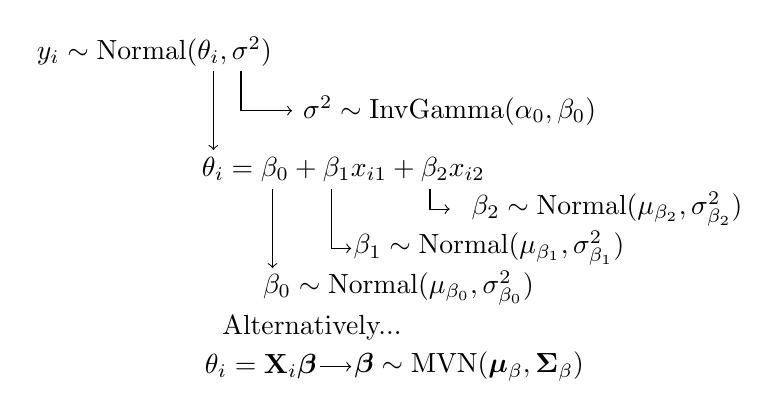
\begin{tikzpicture}
  \node at (0,0) {$y_i \sim \mathrm{Normal}(\theta_i, \sigma^2)$} ;
  	\draw[->] (0.75,-0.25) -- (0.75,-1.25);
  	\node at (2.4, -1.5) {$\theta_i = \beta_0 + \beta_1x_{i1} + \beta_2x_{i2}$};
  		\draw[->] (3.50, -1.75) |- (3.75, -2.00);
  		\node at (5.75, -2) {$\beta_2\sim \mathrm{Normal}(\mu_{\beta_2},\sigma^2_{\beta_2})$};
  		\draw[->] (2.25, -1.75) |- (2.50, -2.50);
  		\node at (4.25, -2.5) {$\beta_1\sim \mathrm{Normal}(\mu_{\beta_1},\sigma^2_{\beta_1})$};
  		\draw[->] (1.50, -1.75) -- (1.50, -2.75);
		\node at (3.1, -3) {$\beta_0\sim \mathrm{Normal}(\mu_{\beta_0},\sigma^2_{\beta_0})$};
		
	\node at (2, -3.5) {Alternatively...};
	\node at (1.35, -4) {$\theta_i = \mathbf{X}_i{\bm\beta}$};
		\draw[->] (2.1, -4) -- (2.5, -4);
		\node at (4, -4) {${\bm\beta}\sim \mathrm{MVN}({\bm\mu}_{\beta},{\bm\Sigma}_{\beta})$};		
  	\draw[->] (1.1, -0.25) |- (1.75, -0.75);
  	\node at (3.75, -0.75) {$\sigma^2\sim \mathrm{InvGamma}(\alpha_0, \beta_0)$};
\end{tikzpicture}

\end{document}